\documentclass[9pt,twocolumn,twoside]{gsajnl}
% Use the documentclass option 'lineno' to view line numbers



\articletype{inv} % article type
% {inv} Investigation 
% {gs} Genomic Selection
% {goi} Genetics of Immunity 
% {gos} Genetics of Sex 
% {mp} Multiparental Populations

\title{Analysis of a TCGA RNA-seq data set on lung squamous cell carcinoma}

\author[$\ast$,1]{Carbonell Gamón, Gabriel}
\author[$\ast$,1]{Matabacas Enebral, Aleix}
\author[$\ast$,1]{McKitrick, Austin}

\affil[$\ast$]{Master Programme on Bioinformatics for Health Sciences, Universitat Pompeu Fabra, Barcelona, Spain}

\keywords{lung cancer; non-small cell lung cancer; transcriptomics; squamous cells; differential expression, gene ontology, TCGA}

\runningtitle{GENETICS Journal} % For use in the footer 

%% For the footnote.
%% Give the last name of the first author if only one author;
% \runningauthor{FirstAuthorLastname}
%% last names of both authors if there are two authors;
% \runningauthor{FirstAuthorLastname and SecondAuthorLastname}
%% last name of the first author followed by et al, if more than two authors.
\runningauthor{Carbonell \textit{et al.}}

\begin{abstract}

%Lung cancer is the most lethal type of cancer in the current times, the most common class are the non-small cell lung cancer, and within them, the lung squamous cell carcinoma (LUSC) is one of the most common due their strong relationship with the smoking habits. Unfortunately, lacks of early diagnostic tools and treatment options. In order of solve that, due the accessibility of obtain microRNA data in the clinical context, most research has focused on analyzing RNA expression profiles on smoker and non-smoker samples. The aims of this study was to analyze this profiles from patients with LUSC and without it, in order to find differently expressed genes heavily involved in LUSC cancer related pathways without taking in account the smoking status. The results of our analysis suggest than the deferentially expressed gens at genom-wide significance found between cancer and non-cancer samples were heavily involved in signal processing and cell metabolism. The gens and pathways found in this study, could be useful starting points in the search of biomarkers for the diagnostic and treatment of LUSC.


Lung cancer, including lung squamous cell carcinoma, is the most lethal type of cancer and lacks early diagnostic tools and treatment options. Research to understand the genes and biological pathways involved in this cancer subtype could provide information to solve this problem. The aim of this study was to analyze RNA expression profiles from patients with this specific cancer subtype in order to find differently expressed genes and pathways that are relevant for this disease. To do this, a differential expression analysis and Gene Ontology analysis were conducted on transcriptomic data using a lung squamous cell carcinoma dataset from The Cancer Genome Atlas project, in which healthy and tumor tissue samples from the same patients were compared. The results of this study showed that 1451 genes were significantly differentially expressed. The subsequent functional analysis suggested that those differentially expressed genes found between cancer and non-cancer samples were heavily involved in signal transduction and cell metabolism. These genes and pathways could be useful starting points to accelerate diagnostics and improve treatments for lung squamous cell carcinoma.
\end{abstract}

\begin{document}

\maketitle
\thispagestyle{firststyle}
\marginmark
\firstpagefootnote
\correspondingauthoraffiliation{gabriel.carbonell01@estudiant.upf.edu, aleix.matabacas01@estudiant.upf.edu, austin.mckitrick01@estudiant.upf.edu}
\vspace{-11pt}%

%\lettrine[lines=2]{\color{color2}T}{}his \textit{Genetics} journal template is provided to help you write your work in the correct journal format. Instructions for use are provided below. 

%\section{Guide to using this template in Overleaf}

%This template is provided to help you prepare your article for submission to the \textit{Genetics}.

% \section{Your Abstract}

% In addition to the guidelines provided in the example abstract above, your abstract should:

% \begin{itemize}
% \item provide a synopsis of the entire article;
% \item begin with the broad context of the study, followed by specific background for the study;
% \item describe the purpose, methods and procedures, core findings and results, and conclusions of the study;
% \item emphasize new or important aspects of the research;
% \item engage the broad readership of GENETICS and be understandable to a diverse audience (avoid using jargon);
% \item be a single paragraph of less than 250 words;
% \item contain the full name of the organism studied;
% \item NOT contain citations or abbreviations.
% \end{itemize}

\section{Introduction}

Among all cancer types, lung cancer is the most lethal among both males and females , being responsible for 28\% of cancer-related deaths \citep{WorldCancerReport}. The life expectancy for those who have lung cancer is very poor and usually is not diagnosed until the cancer's advanced phase. In addition to a late diagnosis, research has shown that patients only have a 16\% survival rate after 5 years of their diagnosis \citep{LungStudy}.

One of the most common types of lung cancer is lung squamous cell carcinoma (LUSC), which typically occurs in the larger bronchi of the lung. Although smokers have a high prevalance of LUSC, non-smokers can suffer this disease too \citep{park2017gab2}. This is a non-small cell lung cancer, which has been found to respond poorly to radiotherapy and chemotherapy in comparison to other kinds of cancer \citep{NCI}. The most common treatment is surgery, which is highly invasive to the patient and doesn't always cure the cancer. An early diagnosis of this cancer could allow for early treatment making the need for surgery avoidable.

Considering these factors, research to characterize the genes and pathways related to LUSC and to increase the prediction and diagnosis capacity is necessary. Previous studies on this topic show the existence of biomarkers that may be used for diagnostic and prognostic purposes, as well as molecular targets for the treatment of this group of cancer \citep{xiao2018identification, hayes2014micrornas}. Unfortunately, this study lacked sensibility in the detection of sub-types of cancer, as it targeted all non-small lung cell carcinomas. 

Therefore, the present study aimed to contribute to the characterization of lung squamous cell carcinoma. Using data profiled from The Cancer Genome Atlas (TCGA), RNA expression profiles were analyzed from patients with LUSC in order to find differently expressed genes and pathways that are relevant for this disease, setting the basis to develop diagnostics and improve treatments.


\section{Materials and Methods}
\label{sec:materials:methods}

\subsection{Data Collection}

Data was obtained from The Cancer Genome Atlas program (TCGA) \citep{atlas}. The data consisted of a table of raw counts containing 20115 genes and 553 samples, organized as a \textit{SummarizedExperiment} object. Of those samples, 502 belonged to tumor tissue and 51 to normal tissue.

\subsection{Statistical Analysis Design}

Data analyses were performed using the R programming language, supported by open source packages from the Bioconductor project. Specific versions used for this study can be found under the \textit{Session information} \citep{se} sections from the \textit{Supplementary Materials}. The data was read using the \textit{SummarizedExperiment} package, and most plots were created with \textit{geneplotter} \citep{geneplotter}. The analysis focused on studying the differences between paired normal and tumor samples. For this, the data set was subsetted by filtering for those samples whose patient code was the same.

\subsection{Quality Assessment and Normalization}

After filtering, data quality was assessed and normalization procedures were applied. This required the transformation of the \textit{SummarizedExperiment} object into a \textit{DGElist} object by means of the \textit{edgeR} package \citep{edger1, edger2}. Changes were kept in sync for both object types. Within-sample normalization was achieved by calculating the counts per million (CPM), which were then log2 transformed. Next, the distributions of library sizes and expression levels among samples and expression levels among genes were examined visually with plots. Based on the later one, genes below 1 logCPM were considered lowly-expressed and were filtered out. Between-sample normalization was done by calculating normalization factors with \textit{edgeR}, and the results of this step were assessed with MA plots. Possible batch effect sources were analyzed by examining the distribution of the elements of the TGCA barcode across samples as surrogate variables. Elements for which a suspicious distribution was found were analyzed by means of hierarchical clustering and multidimensional scaling plot. This visualization was done by removing tumor samples from portion analytes which did not have any normal samples avoiding zeros in the cross-reference table of the outcome of interest and the portion analyte. Normal pairs of these samples were also removed from other portion analytes for the visualization. Samples that did not meet the quality criteria were discarded.

\subsection{Differential Expression Analysis}

The \textit{limma-voom} pipeline from the \textit{limma} package \citep{limma} was used to perform differential expression analysis. A linear model consisting of the type of sample as the outcome of interest and adjusting for the paired design of the analysis by using the patient ID were created. No further adjustments for any known effect were done to the model. The \textit{sva} package \citep{sva} was used to estimate surrogate variables as indicators of unknown variability, which were then added to the model. The performance of statistical tests was assessed with their distributions of raw p-values and moderated t-statistics. After the statistical test, a false discovery rate (FDR) of 1\% was used for type I error correction, and only those genes below that threshold and with a low fold change higher than two or lower than minus two were considered differentially expressed. The differential expression analysis results were diagnosed with volcano and MA plots built using \textit{limma}.

\subsection{Gene Set Enrichment Analysis}

Gene set enrichment analysis (GSEA) was completed using the \textit{GSEABase} package \citep{GSEA} and the C2 collection from the Broad Institute's \textit{MSigDB} gene set collections was used for the analysis. The collection was imported using the \textit{GSVAdata} package \citep{GSVAdata}, and contained 29340 genes and 3272 curated computational gene sets. The analysis calculates an enrichment score for each gene set, which provides information on the changes in gene expression by individual genes in the gene set.

After the individual identifiers in the C2 gene sets and the data set being analyzed were properly mapped to one another, an incidence matrix was created. This matrix indicated what individual genes belonged to the gene sets and the data set being analyzed. A \textit{1} denoted that the gene was a member of that data set, while a \textit{0} denoted that the gene was not a part of that data set. After this, all genes that were not part of data set, or had a \textit{0}, were discarded. 

SVA was then conducted with the same procedure outlined previously. The generated t-statistics were stored in a vector structure and the z-scores were calculated to identify shifts in gene expression within a gene set. A filter was completed to remove genes sets containing less than 5 genes. Finally, a one sample z-test was calculated and a conservative multiple testing adjustment was administered to find if any gene sets were candidates for differentially expressed genes.

\subsection{Gene Set Variation Analysis}

In addition to the GSEA, a gene set variation analysis (GSVA) was performed with the package \textit{GSVA} \citep{GSVA}. This differed from the GSEA previously administered by utilizing a gene set by sample matrix rather than a gene by sample matrix. This matrix was also created with the number of gene sets containing five or more genes and an enrichment score that indicated sample-wise gene-level summaries of expression. The enrichment scores were then used for gene expression values in the differential expression analysis. The genes that were differentially expressed at 1\% FDR were then identified. 
 
\subsection{Gene Ontology Analysis}

Using the differentially expressed genes identified in the differential expression analysis, a Gene Ontology analysis was performed with the package \textit{GOstats} \citep{gostats}. A parameter object was built that specified the gene universe of interest, the set of differentially expressed genes, the ontology, and other information. The ontology selected was \textit{BP}, which matched genes to the Biological Processes associated with the GO Terms. A conditional test was completed and the output was filtered by gene sets containing between 5 and 250 genes. In addition, GO Terms with an Odds Ratio of 1.5 or greater.

\subsection{Data Availability}

The transcript reads used in this analysis can be obtained from the The Genome Cancer Atlas project website. The code used for all the analysis is provided in the supplementary materials, as well as the resulting files of the different filtering steps and analyses under the \textit{results} directory.

\section{Results and Discussion}

\subsection{Quality Assessment}

The data set consisted of 20115 genes, 51 tumor samples and 502 normal samples; but after filtering for those samples which were paired, the number was reduced to 102 samples, maintaining the same number of genes. Two normalization steps were needed to analyze the data: within-sample normalization, to compare across features in a sample, and between-sample normalization to compare a feature across samples. Within-sample normalization was log-transformed to improve the distributional properties. The library size distribution, displayed in the \textit{Figure 1} from the Supplementary Materials, showed a not uniform sequencing depth in which tumor and normal samples were randomly distributed. Gene expression across samples was explored with MDS plots (Supplementary Materials \textit{Figure 2}) for tumor and normal samples separately, without showing any significant problem.

The distribution of expression levels among genes (Supplementary materials \textit{Figure 3}) motivated to set a minimum threshold of expression of 1 log CPM to prevent downstream artifacts in further analyses. After filtering out those genes below that threshold, 11872 genes and 102 samples remained.

After normalization of the data, expression-level dependent biases were checked using MA plots (Supplementary Materials, Figures 4 and 5), which were not observed in either normal or tumor samples in significant levels. The tumor sample from patient \textit{8623} showed in the plot that it was the most different from the average of the others.

Although the portion of analyte stood out as a potential batch effect source, the hierarchical clustering performed with 78 samples showed that those were clustering primarily by type, with the different portions present in both clusters (Supplementary Materials, Figure 6). This reduction of the number of samples was done in order to avoid having zeros in the cross-classification of the outcome of interest with the portion analyte. The resulting plots led to the consideration that this variable was not inducing batch effect. In any case, it was observed that the tumor sample from patient \textit{8623} clustered along the normal samples. The sample was then discarded based on this observation and its MA plot, and its normal pair was also discarded to keep the paired design, leaving a total of 100 samples and 11872 genes. Errors in the annotation of this sample could be the reason for this behaviour, but as there was no access to data prior to annotation, no more insight on the reasons could be provided.

\subsection{Differential Expression Analysis}

The \textit{sva} package estimated 12 surrogate variables, which represent unknown sources of variation. The number of variables could be reduced by fine tuning the model, requiring more analysis of the phenotypical variables present in the data. After including the variables into the model, the \textit{limma-voom} pipeline estimated 9137 significantly expressed genes under a FDR cutoff of 1\%. Of this genes, only those which logarithmic fold change was over two or below minus two were considered for further analysis, leaving 1451 genes being called differentially expressed, of which 896 were down-regulated and 555 up-regulated.

Performance of the statistical test done by means of the distribution of raw p-values, shown at Figure \ref{fig:pval}, and a QQ plot of the moderated t-statistics (Supplementary Materials, Figure 11) showed that diagnoses where correct. The distribution of raw p-values was uniform except for a peak at low p-values, which corresponded to the differentially expressed genes, while the QQ plot showed that most genes were far from the diagonal, showing the significance and amount of the discovered differentially expressed genes.

Regarding the chromosome distribution of those differentially expressed genes passing both the 1\% FDR and the log fold change cutoffs, it did not correspond to a distribution based on the chromosome size. This also acts as an indicator of the quality of the results, as a distribution ordered by size is not expected. Chromosomes with more genes related to processes that are biologically relevant for the context of cancer are expected to rank higher. In this case, chromosomes 1, 19 and 11 were on the top of the ranking (Supplementary Materials, Figure 10).

\begin{figure}[htbp]
\centering
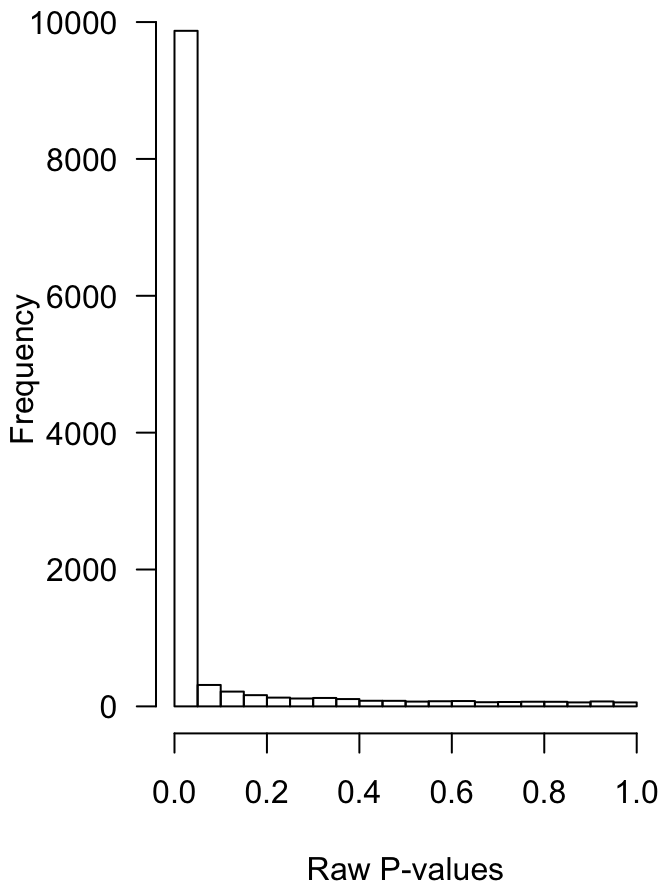
\includegraphics[width=65mm, scale=0.75]{pval}
\caption{\textbf{Raw p-values for the differential expression analysis results.} The figure shows a uniform distribution for not differential expressed genes, which is expected under the null hypothesis, while there is a peak at low p-values for the truly DE genes.}
\label{fig:pval}
\end{figure}

Finally, the results were diagnosed by means of a volcano plot, shown in Figure \ref{fig:de-volcano}. It displays the significance of each gene against its level of differential expression, and no unexpected trends are found.

\begin{figure}[htbp]
\centering
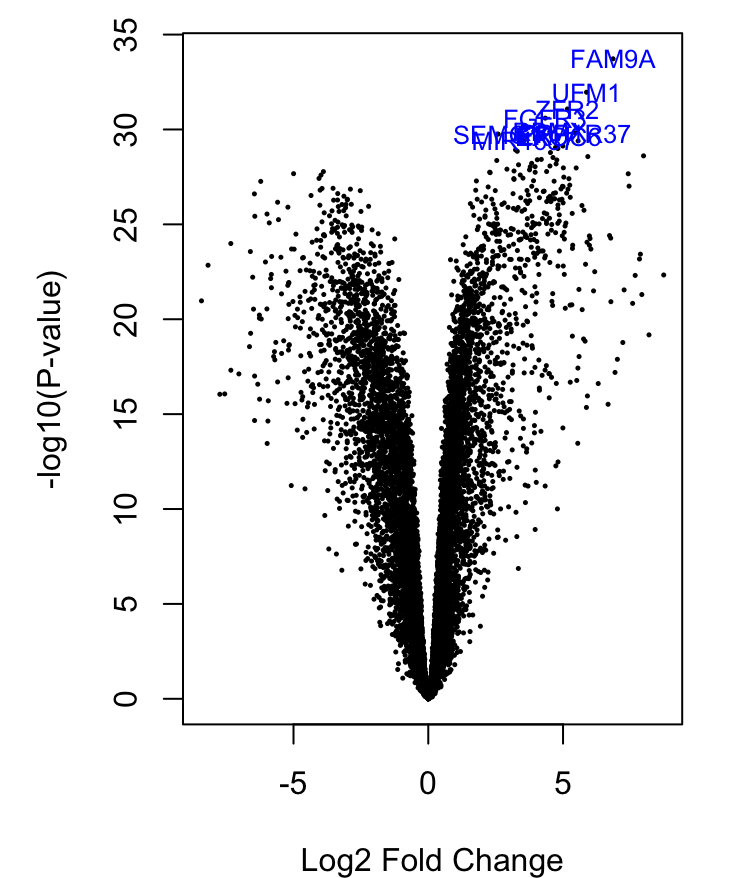
\includegraphics[width=\linewidth-50, scale=0.75]{volcano}
\caption{\textbf{Volcano plot of the differential expression analysis results.} Base 10 log-transformed \textit{p-values} are shown in the \textit{y} axis as a measure of significance, while the base 2 logarithm of the fold change is shown in the \textit{x} axis as a measure of the differential expression level. The top 10 differentially expressed genes are labeled. Labels are: FAM9A, UFM1, ZFR2, FGFR3, RBMX, SEMG1, PPP1R37, ERH, EXOC6, MIR4687.}
\label{fig:de-volcano}
\end{figure}

\subsection{Gene Set Enrichment Analysis}

Functional enrichment analysis techniques, such as a GSEA, are valuable tools since they have the ability to detect sensitive and small changes in differential expression at the gene set level. Although 1451 differentially expressed genes were obtained from the differential expression analysis, tests of functional enrichment were explored to compare differences among techniques.

After mapping the C2 data and the data being analyzed, 9963 genes among 100 samples were left for the SVA portion of the GSEA. After conducting a SVA and filtering out gene sets with less than 5 genes, 9963 genes among 2760 gene sets were left from the original 3272 of the C2 collection. A one sample z-test and a conservative multiple testing adjustment was conducted and 2313 gene sets were showed to be differentially expressed.

\subsection{Gene Set Variation Analysis}

In addition, a GSVA was completed as part of the functional enrichment analysis. This differed from the GSEA previously administered by utilizing a gene set by sample matrix rather than a gene by sample matrix, which allows for the pathway enrichment for each individual sample to be analyzed. After the data was normalized and properly filtered, the GSVA found 1877 gene sets to be differentially expressed at 1\% FDR. 

Techniques such as GSEA and GVSA are often used only when differentially expressed genes are not found in the DE analysis. Since this study identified 1451 differentially expressed genes in the DE analysis, these genes were selected to complete the GO analysis. Results on GSVA and GSEA are given as preliminary, as the proper analysis of the enriched sets was not performed yet. A possible future direction could explore the GO analysis using the gene sets found in the GSEA and GVSA from this study.

\subsection{Gene Ontology Analysis}

To extract knowledge from the RNA expression profiles, the usage of algorithms to detect DE genes is not enough \citep{dudoit2002statistical}. The biological function of the detected genes should be studied in order to know what functions and pathways are altered. In this sense, the Gene Ontology Consortium  homogenizes the format and vocabulary of the biological data obtained from research to make it reusable\citep{GO}. This allowed for the use of the obtained differentially expressed genes as a query in its database, reducing the amount of experimental studies and accelerating research.

After performing a conditional test and the appropriate filtering, 33 GO Terms were identified. The specific differentially expressed genes associated with each GO Term were identified as well. The results of the GO analysis suggested that the differentially expressed genes discovered in this study were highly involved in signal transduction. Cancer samples had differentially expressed genes associated with signal complex assembly (OR = 27.78, P = 1.14x10-3), the collagen-activated tyrosine kinase receptor signaling pathway (OR = 9.26, P = 6.44x10-3), and adenylate cyclase-activating G protein-coupled receptor signaling pathway (OR = 2.64, P = 5.21x10-4) in comparison to normal samples. Past research using GO analysis has found the parent GO term associated with signal transduction to be significant among the differentially expressed genes studied \citep{long2019identification}. However, this study didn't find the specific child-class GO terms found in the present study. Perhaps the genes controlling for these specific signaling pathways could be helpful in the development of diagnostics and treatment for this kind of lung cancer Table \ref{tab:go-terms} summarizes the highlighed results from the Gene Ontology analysis.

In addition to signal transduction, the differentially expressed genes were also involved in cell activity, mainly cell metabolism. The GO analysis showed cancer samples had differentially expressed genes associated with the negative regulation of mRNA splicing (OR = 4.63, P = 7.26x10-3), and mRNA splice site selection (OR = 4.28, P = 2.81x10-3). Splicing plays an important role in essential biological processes, including cancer, and past research suggests a relationship exists between the dysregulation of mRNA splicing and lung cancer \citep{altsplicing}. Therapeutic approaches that act on the regulation of mRNA splicing could be a helpful in treating lung cancer.

\subsection{Concluding Remarks}

In conclusion, this study successfully identified differentially expressed genes and associated biological pathways unique to LUSC samples in this data. Among those pathways, it appears that signal transduction and cell metabolism were highly enriched. Therefore, the genes involved in these pathways could be important to developing diagnostics and treatments for lung squamous cell carcinoma. 

\section{Acknowledgements}

We would like to thank our instructor Robert Castelo and our classmates for all the help and ideas that they have given us during this project. Also thanks to Eric Climent, our friendly statistician, for helping us with its past experience with RNA-seq experiment results.

\bibliography{bibliography}

\renewcommand{\arraystretch}{3}
\begin{table*}[htbp]
\centering
\caption{ \bf {Highlighted enriched GO terms from differentially expressed genes}}
\begin{tableminipage}{\textwidth}
\begin{tabularx}{\textwidth}{sssssX}
  \hline
  GOBPID\footnote{Excerpt of the complete GO results table found under Supplementary Materials, with highlighted GO terms that were discussed.} & P-value & Odds Ratio & Count\footnote{Number of genes mapped to the gene set} & Size\footnote{Size of the gene set} & Term \\ 
  \hline
GO:0007172 & 1.14x10-3 & 27.78 &   4 &   5 & Signal complex assembly  \\
GO:0038063& 6.44x10-3 & 9.26 &   4 &   7 & Collagen-activated tyrosine kinase receptor signalling pathway  \\ 
GO:0048025 & 7.26x10-3 & 4.63 &   6 &  15 & Negative regulation of mRNA splicing, via spliceosome  \\ 
GO:0006376 & 2.81x10-3 & 4.28 &   8 &  21 & mRNA splice site selection  \\ 
GO:0007189 & 5.21x10-4 & 2.64 &  20 &  73 & Adenylate cyclase-activating G protein-coupled receptor signaling pathway  \\ 
\hline
\end{tabularx}
  \label{tab:go-terms}
\end{tableminipage}
\end{table*}

\end{document}